\documentclass[12pt]{article}
\setlength\parindent{0pt}
\usepackage{fullpage}
\usepackage{amsmath}
\usepackage{graphicx}
\usepackage{lscape}
\setlength{\parskip}{4mm}
\usepackage[margin=0.5in]{geometry}

\begin{document}
\pagenumbering{gobble}

\begin{center}\sc{\Large Frontiers in Science -- Astronomy}\end{center}

Welcome! I'm Walter Freeman, a professor of physics and astronomy at Syracuse. If you ever want to get in touch with me
afterwards, you can email me at {\tt wafreema@syr.edu} or call or text me at (520) 409 3766.

Carl Sagan, a famous astronomer, said ``We are all stardust''. He meant this literally! We are made out of the remains of
exploding, dying stars. We know this by looking at the 
colors of the things that we are made of, looking at the colors of the Sun and the stars, and realizing that they're the same.

Today we're going to learn:

\begin{itemize}
\item ... how we know all this!
\item How the colors of light are a lot more detailed than we can see with our eyes
\item How a machine called a ``spectrometer'' can give us more detail about the colors of light
\item How light relates to chemistry:
\begin{itemize}
\item How each chemical element has its own unique color spectrum fingerprint
\item How to tell what chemical something is by the light it gives off
\item How to calculate the color spectrum fingerprint of any kind of atom, if you know its chemistry
\end{itemize}
\item How light is related to heat
\item How to tell the temperature of stars, and of anything else, by the light it gives off
\item {\bf How to tell what any star is made of by its color}
\item ... and what we learn when we do that!
\end{itemize}

The most important rule is {\it to have fun}! I'm here to answer any questions you have; we have more nifty stuff
for you to do and to experience than you have time for, so choose whatever is most interesting to you. 



Some rules for your safety and for the safety of the equipment: 

\begin{itemize}
\item Don't leave the discharge tubes on for more than 5 minutes at a time
\item Be careful of the power cables
\item Be gentle with the computer spectrometers
\item You all can use the infrared camera, but {\bf only if one of the guides is standing right next to you}
\end{itemize}

\newpage

Some terms you will learn (they're just here for reference -- don't worry about memorizing them!):

\begin{itemize}
\item {\bf Light:} Any kind of electromagnetic radiation, even the ones we can't see: radio, microwave, infrared, ultraviolet...
\item {\bf Photon:} A single tiny particle of light. The lights in this room spit out 100 trillion trillion photons a second!
\item {\bf Electron volt:} A tiny unit of energy, good for measuring tiny things, like photons
\item {\bf Chemical element:} A type of atom. Elements are things like hydrogen, helium, oxygen, neon, sodium, mercury, iron, lead, gold, and so on.
\item {\bf Energy level:} Atoms can have different amounts of energy. Each chemical element only has a few very specific amounts of energy that it can have, called {\it energy levels}.
\item {\bf Emission:} An atom in a higher energy level can go down to a lower energy level and produce a photon.
\item {\bf Absorption:} An atom in a lower energy level can go up to a higher energy level and absorb a photon.
\item {\bf Thermal radiation:} Hot things produce photons of many different energies. As a thing gets hotter, the average photon
energy goes up (``the light gets bluer''), and the number of photons goes up (``the light gets brighter'').
\end{itemize}

\bigskip
\begin{center}
\Large This reference will be helpful!

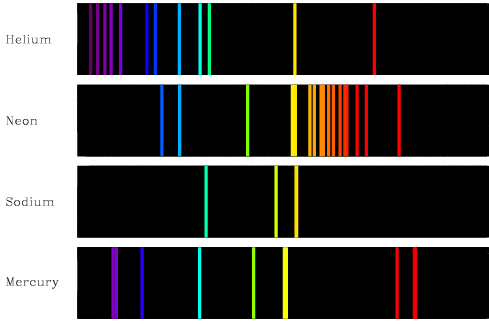
\includegraphics[width=0.6\textwidth]{spectra.png}

(Hydrogen is not on here -- you'll have to figure it out on your own!)
\end{center}
\newpage

\begin{minipage}{0.1\textwidth}
\begin{center}
\Large Front \\ Right
\end{center}
\end{minipage}
\begin{minipage}{0.8\textwidth}
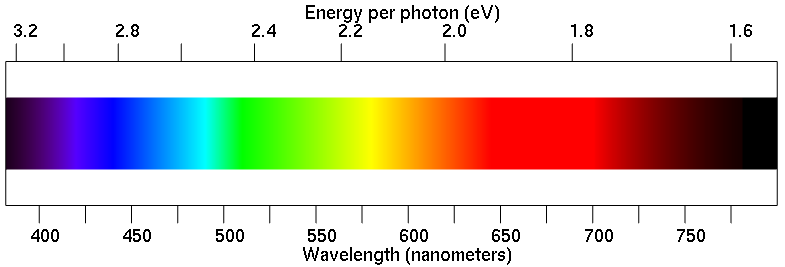
\includegraphics[width=\textwidth]{spectrum2.png}
\end{minipage}

\begin{minipage}{0.5\textwidth}
What color does this appear?
\end{minipage}
\begin{minipage}{0.5\textwidth}
What element is it?
\end{minipage}


\vspace{1in}
\hrule

\begin{minipage}{0.1\textwidth}
\begin{center}
\Large Front \\ Left
\end{center}
\end{minipage}
\begin{minipage}{0.8\textwidth}
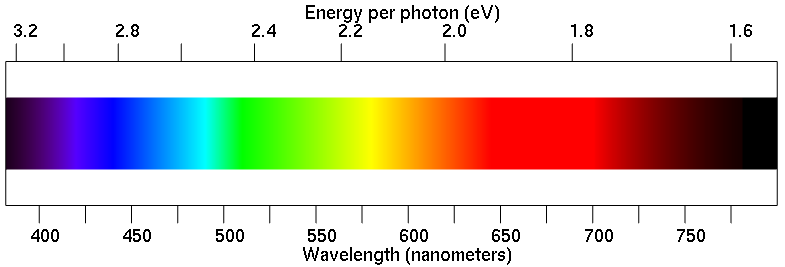
\includegraphics[width=\textwidth]{spectrum2.png}
\end{minipage}

\begin{minipage}{0.5\textwidth}
What color does this appear?
\end{minipage}
\begin{minipage}{0.5\textwidth}
What element is it?
\end{minipage}

\vspace{1in}
\hrule

\begin{minipage}{0.1\textwidth}
\begin{center}
\Large Rear \\ Right
\end{center}
\end{minipage}
\begin{minipage}{0.8\textwidth}
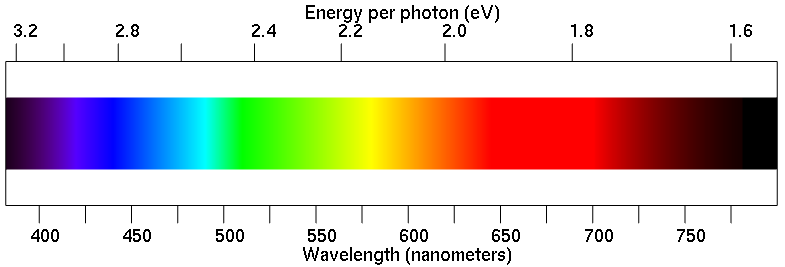
\includegraphics[width=\textwidth]{spectrum2.png}
\end{minipage}

\begin{minipage}{0.5\textwidth}
What color does this appear?
\end{minipage}
\begin{minipage}{0.5\textwidth}
What element is it?
\end{minipage}
\newpage

\begin{minipage}{0.1\textwidth}
\begin{center}
\Large Rear \\ Left
\end{center}
\end{minipage}
\begin{minipage}{0.8\textwidth}
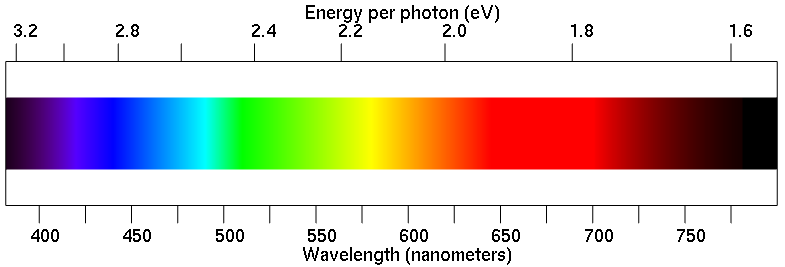
\includegraphics[width=\textwidth]{spectrum2.png}
\end{minipage}

\begin{minipage}{0.5\textwidth}
What color does this appear?
\end{minipage}
\begin{minipage}{0.5\textwidth}
What element is it?
\end{minipage}


\vspace{1in}
\hrule

\begin{minipage}{0.1\textwidth}
\begin{center}
Shaded\\Lamp
\end{center}
\end{minipage}
\begin{minipage}{0.8\textwidth}
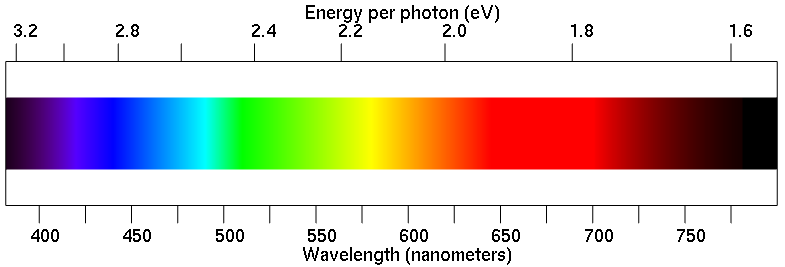
\includegraphics[width=\textwidth]{spectrum2.png}
\end{minipage}

\begin{minipage}{0.5\textwidth}
What color does this appear?
\end{minipage}
\begin{minipage}{0.5\textwidth}
What element is it?
\end{minipage}

\vspace{1in}
\hrule

\begin{minipage}{0.1\textwidth}
\begin{center}
Vertical \\ Bulb
\end{center}
\end{minipage}
\begin{minipage}{0.8\textwidth}
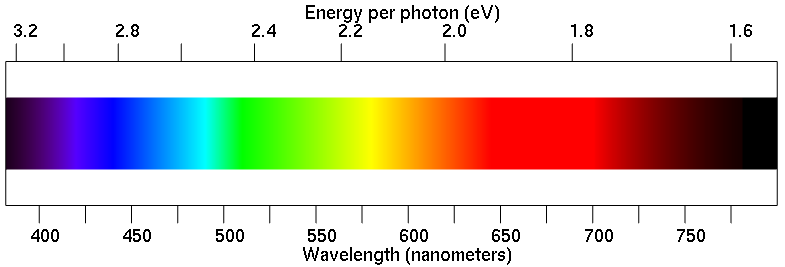
\includegraphics[width=\textwidth]{spectrum2.png}
\end{minipage}

\begin{minipage}{0.5\textwidth}
What color does this appear?
\end{minipage}
\begin{minipage}{0.5\textwidth}
What element is it?
\end{minipage}

\newpage
\begin{landscape}

\begin{center}
\Large 
Predicting the Colors of Hydrogen
\end{center}

\large 
You may have learned in your chemistry class about {\it atomic energy levels}. In general, the formula for the energy levels of atoms is very complicated (and there are lots and lots of them!)

But hydrogen is simple. Its energy levels follow a pattern:

$$\text{Energy of level n} = 13.6 \times \frac{n^2-1}{n^2} \text{ electron volts (eV)}.$$

We name these levels by writing $n=$ and then a number. So $n=1$ is the lowest, $n=2$ is the next one, and so on.

An ``electron volt'' is just a very small amount of energy useful for talking about atoms. There are 26 thousand trillion trillion ($2.6 \times 10^{22}$) eV in a food-Calorie.

The law of conservation of energy tells us how atoms changing energy levels will relate to light:


\begin{itemize}
\item If an atom jumps to a {\bf higher} energy level, it needs to {\bf take} energy from something, and so it must  {\bf absorb} a photon with energy equal to the difference
\item If an atom jumps to a {\bf lower} energy level, it needs to {\bf give} energy to something, and so it must {\bf produce} a photon with energy equal to the difference
\end{itemize}

Remember that each color goes with photons of a specific energy. So this means:

{\bf If you know the energy levels of an atom, you can figure out its color spectrum fingerprint by calculating all 
the different differences between them!}

\newpage
Below, I've given you the amounts for the first five energy levels of hydrogen. You can fill out the table and predict the colors that hydrogen can emit and absorb. Label those colors on the spectrum with your pencil... then find the hydrogen lamp in this room
and see if it matches!

\bigskip

\large
\begin{tabular}{|c|c|c|c|c|c|c|c|c|}
\hline
Higher energy level (to the right) & \multicolumn{2}{c|}{\textbf{\begin{tabular}[c]{@{}c@{}}n=5\\ 13.1 eV\end{tabular}}} & \multicolumn{2}{c|}{\textbf{\begin{tabular}[c]{@{}c@{}}n=4\\ 12.8 eV\end{tabular}}} & \multicolumn{2}{c|}{\textbf{\begin{tabular}[c]{@{}c@{}}n=3\\ 12.1 eV\end{tabular}}} & \multicolumn{2}{c|}{\textbf{\begin{tabular}[c]{@{}c@{}}n=2\\ 10.2 eV\end{tabular}}} \\ \hline
Lower energy level (below)         & Energy                                    & Color                                   & Energy                                   & Color                                    & Energy                                   & Color                                    & Energy                                   & Color                                    \\ \hline
\textbf{n=1, 0 eV}                 & 13.1-0=13.1                               & Ultraviolet                             &                                          &                                          &                                          &                                          &                                          &                                          \\ \hline
\textbf{n=2, 10.2 eV}              &                             &                                   &                                          &                                          &                                          &                                          & -                        & -                        \\ \hline
\textbf{n=3, 12.1 eV}              &                              &                                 &                                          &                                          & -                        & -                        & -                        & -                        \\ \hline
\textbf{n=4, 12.8 eV}              & 13.1-12.8=0.3                             & Infrared                                & -                        & -                        & -                        & -                        & -                        & -                        \\ \hline
\end{tabular}

\bigskip

\begin{minipage}{1in}
\large
$E > 3.2$ eV\\
Ultraviolet
\end{minipage}
\begin{minipage}{8in}
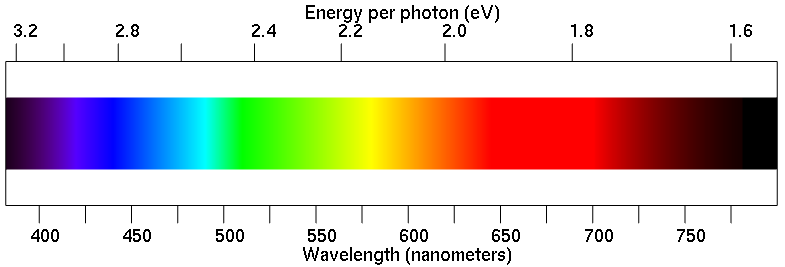
\includegraphics[width=\textwidth]{spectrum2.png}
\end{minipage}
\begin{minipage}{1in}
$E < 1.6$ eV\\
Infrared
\end{minipage}
\end{landscape}

\newpage

\begin{center}\Large Detective Work: What's In The Sign?\end{center}

The ``Experience Physics'' sign on the first floor has four different colors: pink, white, blue, and red. Based on what you
did before, what elements are they? Three of them are the same element; which one?

(Remember, colored glass can't create any new lines that weren't already there -- it can only remove colors!)

 \begin{minipage}{0.1\textwidth}
\begin{center}
``Experi-\\ence''
\end{center}
\end{minipage}
\begin{minipage}{0.8\textwidth}
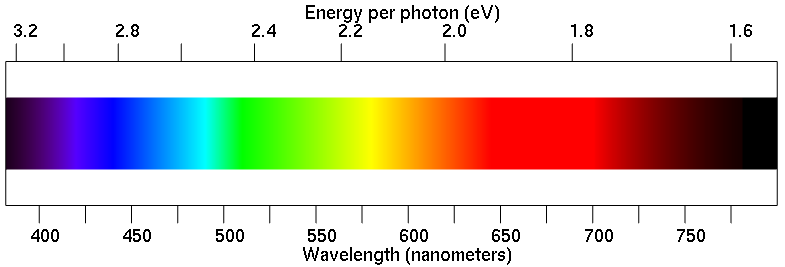
\includegraphics[width=\textwidth]{spectrum2.png}
\end{minipage}

\begin{minipage}{0.5\textwidth}
What color does this appear?
\end{minipage}
\begin{minipage}{0.5\textwidth}
What element is it?
\end{minipage}


\vspace{0.7in}
\hrule

\begin{minipage}{0.1\textwidth}
\begin{center}
\large ``Physics''
\end{center}
\end{minipage}
\begin{minipage}{0.8\textwidth}
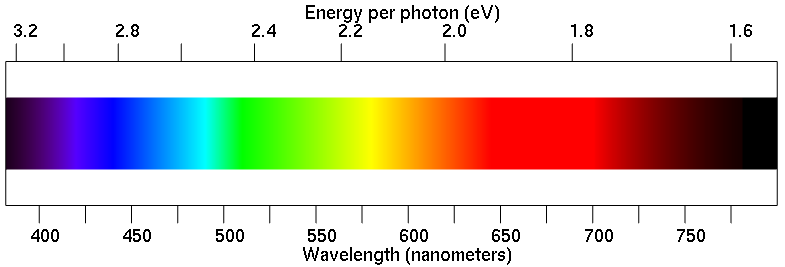
\includegraphics[width=\textwidth]{spectrum2.png}
\end{minipage}

\begin{minipage}{0.5\textwidth}
What color does this appear?
\end{minipage}
\begin{minipage}{0.5\textwidth}
What element is it?
\end{minipage}

\vspace{0.7in}
\hrule

\newpage

 \begin{minipage}{0.1\textwidth}
\begin{center}
\large Yellow
\end{center}
\end{minipage}
\begin{minipage}{0.8\textwidth}
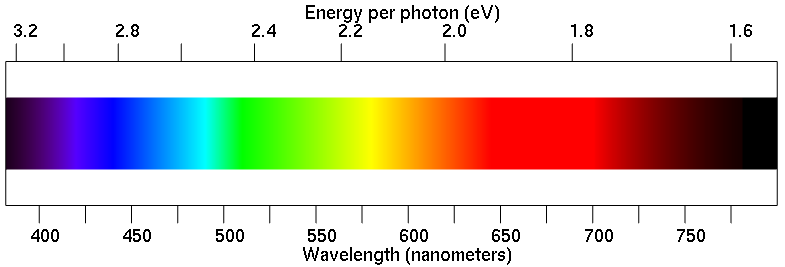
\includegraphics[width=\textwidth]{spectrum2.png}
\end{minipage}

\begin{minipage}{0.5\textwidth}
What element is this?
\end{minipage}
\begin{minipage}{0.5\textwidth}
\end{minipage}


\begin{minipage}{0.1\textwidth}
\begin{center}
\large White
\end{center}
\end{minipage}
\begin{minipage}{0.8\textwidth}
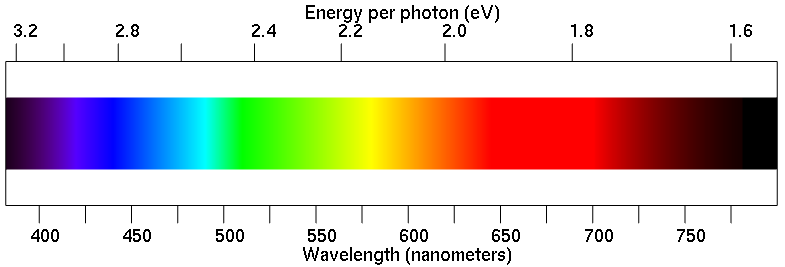
\includegraphics[width=\textwidth]{spectrum2.png}
\end{minipage}

\begin{minipage}{0.5\textwidth}
What element is this?
\end{minipage}
\begin{minipage}{0.5\textwidth}
\end{minipage}

\newpage

\begin{landscape}
\begin{center}
\Large
A detailed spectrum of the Sun.

All the dark lines are the fingerprints of all the different elements in the Sun's atmosphere. These are the same 
elements we have here on Earth!

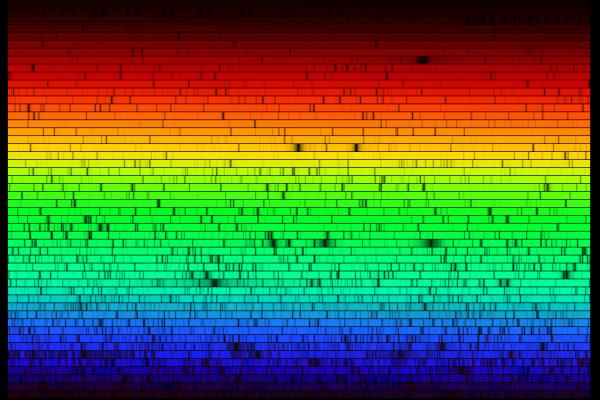
\includegraphics[width=9in]{solarspectrum.jpg}
\newpage
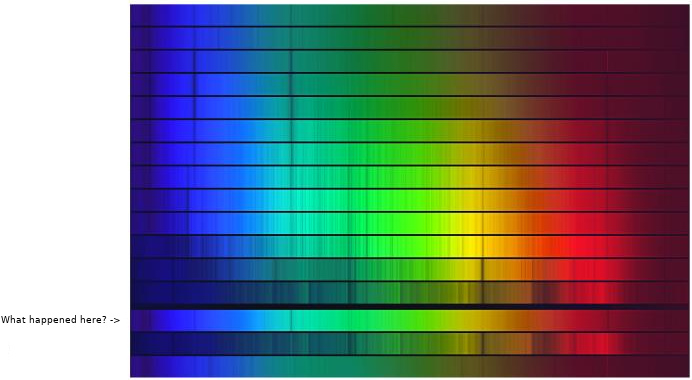
\includegraphics[width=10in]{stellar-spectra.jpg}

\bigskip

What can we tell from the spectra of these stars?

\bigskip

What happened to the one marked by the arrow? 


\end{center}
\end{landscape}

\end{document}
